\section{{\bf Conclusions}}
%\section{{\bf Conclusions \& Outlook}}


%%%%%%%%%%%%%%%%%%%%%%%%%%%%%%%%%%%%%%%%%%%%%%%%%%%%%%%
\begin{frame}{Conclusions}

\begin{mybox}
\begin{wideitemize}
\item 
\end{wideitemize}
\end{mybox}


\vfill

{\footnotesize
{P.~Gatto}, F.~Lipparini, B.~Stamm. ``Computation of Forces arising from the Polarizable Continuum Model within the Domain-Decomposition Paradigm.'' Submitted to \textit{Journal of Chemical Physics}.
}
\end{frame}

%%%%%%%%%%%%%%%%%%%%%%%%%%%%%%%%%%%%%%%%%%%%%%%%%%%%%%%%
%\begin{frame}{Outlook}
%
%
%\begin{mybox}
%\begin{wideitemize}
%
%\item Develop a strategy to automatically construct a competitive partitioning through a graph partitioner the employs grid information;
%\item Further investigate the applicability of the preconditioner: different types of discretizations, time-varying problems, etc.;
%
%\item Study the resilience of the preconditioner.
%
%\end{wideitemize}
%\end{mybox}
%
%\end{frame}


%%%%%%%%%%%%%%%%%%%%%%%%%%%%%%%%%%%%%%%%%%%%%%%%%%%%%%%%
%\begin{frame}{Computational Fluid Dynamics}
%
%\begin{columns}
%\begin{column}[c]{5cm}
%\begin{center}
%\includegraphics[width = 1\textwidth]{figures/cfd.eps}\\
%\texttt{Pres\_Poisson.mat}
%\end{center}
%\end{column}
%
%\begin{column}[c]{5cm}
%\begin{center}
%\includegraphics[width = 1\textwidth]{figures/imatrix_cfd.eps}
%\end{center}
%\end{column}
%
%\end{columns}
%
%
%\end{frame}





%%%%%%%%%%%%%%%%%%%%%%%%%%%%%%%%%%%%%%%%%%%%%%%%%%%%%%%
\section{}
{
\usebackgroundtemplate{
%\tikz\node[opacity=0.45,inner sep=0pt] {\includegraphics[height=\paperheight,width=\paperwidth]{figures/epfl_photo}};}
\tikz\node[opacity=0.35,inner sep=0pt] {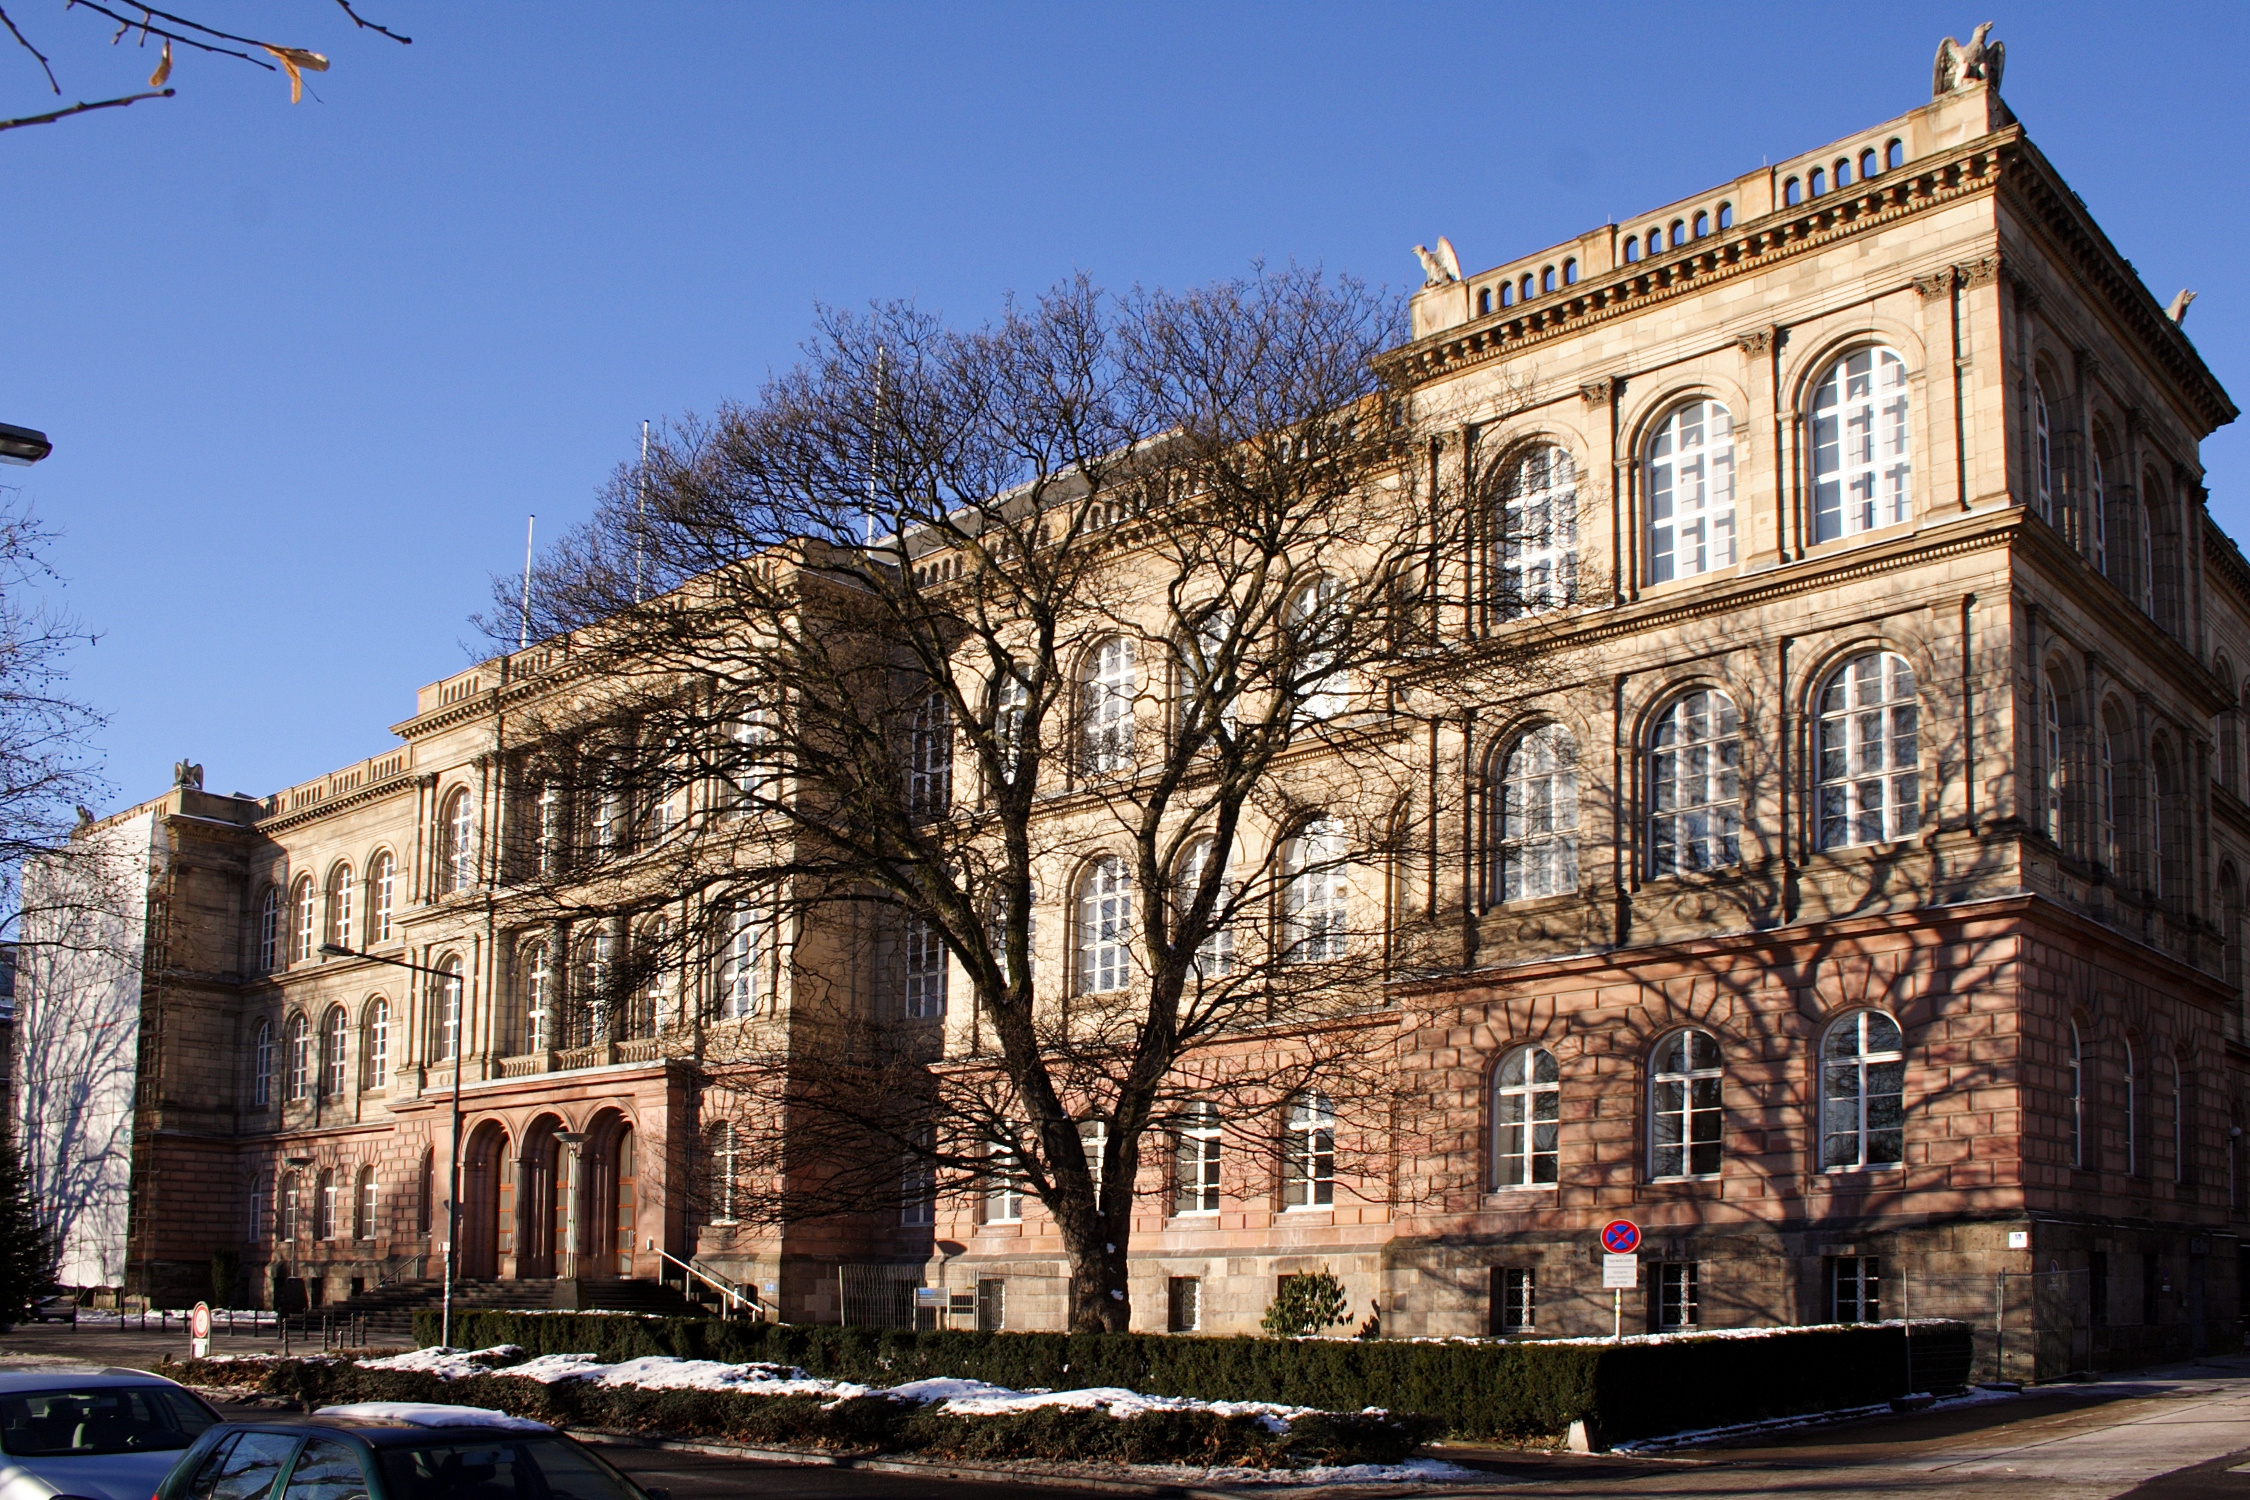
\includegraphics[height=\paperheight,width=\paperwidth]{figures/aachen_background_4}};}
\begin{frame}{}

\vspace{1cm}
\begin{center}
\huge{\bf Thank you!} \\
\vspace{0.5cm}
\large{Questions?}
\end{center}
\end{frame}
}